\documentclass[11pt,a4paper]{article}

\usepackage{polski}
\usepackage[utf8]{inputenc} 
\usepackage{graphicx}
\usepackage {listings}
\usepackage{verbatim}
\title{%
Sprawozdanie Projekt Indywidualny \\
\large Program konwertujący różne systemy liczbowe}
\author{Kamil Sibilski}
\date{16.06.2020}

\begin{document}
\maketitle

\tableofcontents
\newpage

\section{Wprowadzenie}
Celem projektu było stworzenie aplikacji która będzie umożliwiała wygodne zamienianie liczb pomiędzy różnymi systemami liczbowymi.\\
Niestety komputer nie jest w stanie liczyć w naszym (dziesiętnym) systemie liczbowym. Zamiast tego używa systemu binarnego który wykorzystuje tylko 2 znaki. Ze względu na małą liczbę znaków, liczby szybko się stają w tym systemie bardzo długie co utrudnia czytanie ich. Aby to rozwiązać komputer zamienia postać binarną na hexadecymalną, czyli szesnastkową. Jest to o tyle wygodne, że bardzo łatwo jest komputerowi wykonywać zamiany pomiędzy tymi systemami a większa liczba znaków znacznie skraca długość liczb co ułatwia czytanie ich. Na przykład adresy mac kart sieciowych komputer zapisuje w systemie binarnym ale wyświetla w hexadecymalnym bo w pierwszym ma on długość 48 znaków a w drugim tylko 12. Ze względu na te zamiany praca z komputerem na niskim poziomie programowania (sterowania procesorem, obsługą pamięci ram, sterownikami) jest utrudniona bo musimy podawać komendy w tych systemach liczbowych, podczas gdy my operujemy w systemie dziesiętnym. W wyższych warstwach, aby ułatwić korzystanie użytkownikowi, wartości te są zamieniane na liczby dziesiętne lecz na niskich warstwach posiadanie programu/kalkulatora do zamian z naszego systemu liczbowego na "język komputera" jest niemalże niezbędne.\\
Innym ciekawym zastosowaniem systemów liczbowych w informatyce jest indeksowanie rekordów w bazach danych. Aktualnie przy naszych narzędziach informatycznych jesteśmy w stanie tworzyć ogromne bazy danych liczące miliony a nawet miliardy rekordów. Popularne jest aby wszystko indeksować od 1 i iteracyjne zwiększać wartość o 1, czyli pierwszy element ma indeks 1, drugi 2, trzeci 3 itd. Wtedy dokładnie widać ile mamy rekordów w bazie (wystarczy zobaczyć indeks ostatnio dodanego elementu) oraz jest to uporządkowane. Niestety ten system indeksowania posiada sporą wadę. Pozwala on w bardzo prosty sposób osobie z zewnątrz iterować po bazie danych i przez to przeglądać ją całą, dotrzeć do elementów zastrzeżonych/ukrytych lub całkowicie ją zmienić np. za pomocą SQL injection. Rozwiązaniem tego problemu jest używanie większych systemów liczbowych. Jeżeli użyjemy systemu 62 znakowego i ciągu znaków o długości np. 10 to będziemy mieli 839299365868340200 różnych indeksów. Taka ilość pozwala na przypisanie każdemu rekordowi bazy losowej liczby indeksu. Dzięki temu każdy element bazy ma unikalny indeks a szansa na to że w bazie z milionem rekordów ktoś zgadnie index rekordu jest absurdalnie mała. Takie rozwiązanie zapobiega iterowaniu po bazie oraz znacznie utrudnia szukanie elementów prywatnych. Dzięki wysokiemu systemowi liczbowemu możemy użyć tylko 10 znaków zamiast 18 co znacznie zmniejszy zużycie pamięci. Takie właśnie rozwiązanie stosuje serwis YouTube. Wszystkie filmy na tym serwisie mają 11znakowy indeks w systemie 64 znakowym. Dzięki temu prawie niemożliwe jest dostanie się losowo na film który jest prywatny, czyli taki który można odtworzyć znając wyłącznie ten indeks.\\
Teraz kiedy już wiemy dlaczego potrzebne są różne systemy liczbowe, te duże i małe, przejdźmy do aplikacji która ułatwia zamianę systemów liczbowych oraz pozwala na lepsze poznanie ich możliwości.

\section{Obsługa aplikacji}
\begin{center}
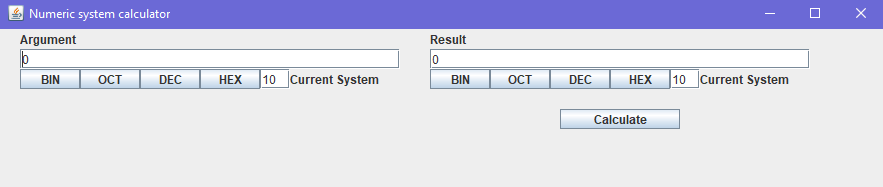
\includegraphics[scale=0.4]{Aplication.png}
\end{center}
Aplikacja została napisana w języku Java oraz wyeksportowana do pliku .jar dlatego aby z niej korzystać potrzeba zainstalować Java RE. Po uruchomieniu pojawia nam się ekran główny. Składa się on z dwóch części, lewej odnoszącej się do wpisywanej przez nas wartości oraz prawej służącej do wyświetlania wyniku. Obie części mogą pracować na różnych systemach liczbowych co pozwana na zamianę dowolnego systemu na inny dowolny. Pod oknem do wpisywania znajdują się przyciski do szybkiego użycia. Zamieniają one systemy liczbowe bez potrzeby wpisywania ich ręcznie. Na prawo od nich znajduje się małe okno do wpisywania które pokazuje aktualnie wybrany system liczbowy oraz pozwala na ręcznie wpisanie dowolnego systemu z zakresu od 2 do 62. Aby uzyskać wynik należy wprowadzić liczbę w okienku argument, następnie wybrać lub wpisać w jakim jest ona systemie(domyślnie 10), na końcu wybrać w jakim systemie chcemy otrzymać wynik(domyślnie 10) i potwierdzić przyciskiem calculate. Jeżeli coś zostało błędnie wprowadzone, aplikacja wyświetli stosowny komunikat. Po tym wszystkim w okienku result powinien się pojawić wynik. Można go bez problemu kopiować. Wszystkie zmiany w trakcie liczenia, np. gdybyśmy chcieli tylko zmienić wyświetlany wynik z 10 na 16, należy zatwierdzać przyciskiem calculate.

\section{Działanie aplikacji}
Aplikacja dzieli się na dwie części. Pierwsza część, główny program, odpowiada za wygląd okna, ustawianie przycisków i wywoływanie funkcji kalkulatora. Druga część, klasa kalkulator, odpowiada za wszystkie działania logiczne jak sprawdzenie poprawności czy zamiana na systemy liczbowe.\\
Główny program został zbudowany z użyciem graficznej biblioteki swing. Znaczna większość współrzędnych jest wprowadzona w formie zmiennych co ułatwia ich łatwe przesuwanie lub stworzenie w przyszłości osobnego okienka do opcji. Głównym elementem jest Frame do którego się dodaje poszczególne elementy typu Button czy TextField.\\
Klasa kalkulator zawiera metody:\\
publiczne:\\
\begin{itemize}
\item checkIfcorrect - sprawdza czy podana wartość jest zgodna z systemem liczbowym. Zwraca prawda jeżeli zgodne
\item checkSys - sprawdza czy system liczbowy jest w zakresie obsługiwanym przez kalkulator. Zwraca prawda jeżeli jest w zakresie
\item convert - zamienia podaną wartość z podanego systemu na inny system. Zwraca przekonwertowaną wartość w formie stringa
\end{itemize}
prywatne:\\
\begin{itemize}
\item convertToDec - zamienia na system dziesiętny. Zwraca wartość w postaci longa
\item decodeSign - zamienia znak na wartość dziesiętną. Zwraca wartość dziesiętną
\item convertToSys - zamienia z systemu dziesiętnego na podany system. Zwraca wynik w postaci stringa
\item codeSign - zamienia wartość dziesiętną na odpowiedni znak. Zwraca zmienną znakową
\end{itemize}

\section{Wnioski}
Projekt uważam za udany. Udało się stworzyć działającą aplikację. Program działa bez zarzutów a jego użytkowanie jest proste i intuicyjne.\\
Największy problemem było stworzenie graficznego interfejsu w swingu. Używanie go jest męczące ze względu na ustawianie sporej ilości ustawień pozycyjnych co bez ciągłego podglądu jest czasochłonne. Stworzenie okna zajęło więcej czasu niż napisanie logiki aplikacji.\\
Wybór javy pod tworzenie logiki aplikacji było dobrym pomysłem. Bez problemu można było manewrować pomiędzy zmiennymi znakowymi a liczbowymi a podział problemu na mniejsze moduły znacząco ułatwiło zrozumienie go i zaimplementowanie.\\
Wybór javy pod tworzenie interfejsu graficznego było słabym pomysłem. Używanie go jest bardzo sztywne a próba konfiguracji pod różne rozmiary okna może się okazać bardzo problematyczne. W przypadku rozwoju tego projektu przydało by się użycie innej biblioteki.\\

\section{Kod źródłowy}
Kod źródłowy aplikacji wraz z aplikacją i sprawozdaniem dostępny jest na repozytorium na GitHub:\\
https://github.com/BridalSkydriver/Projekt-indywidualny
\end{document}

